\begin{note}
    此小节还未完成。
\end{note}

\subsection{滤波器的表示}

\begin{definition}
    \bd{滤波器}是以特定方式改变信号的频率特性,从而变换信号的处理系统。
    滤波器一般有如下类别,如图 \ref{fig:filter_types} 所示:
    \begin{enumerate}[label=(\arabic*)]
        \item 高通滤波器(HP)
        \item 低通滤波器(LP)
        \item 带通滤波器(BP)
        \item 带阻滤波器(BS)
        \item 全通滤波器(AP)
    \end{enumerate}
    \begin{figure}[H]
        \centering
        \includegraphics[width=0.8\textwidth]{chap4/img/filter_types.png}
        \caption{滤波器类型}
        \label{fig:filter_types}
    \end{figure}

    滤波器也可以被分为\bd{模拟滤波器}和\bd{数字滤波器}。
    \begin{itemize}
        \item \bd{模拟滤波器}是由电阻、电容、电感等部件构成的电路。
            滤波器特性对所用部件的物理标称值非常敏感,而且,
            有些部件的物理特性会随温度变化而改变。
        \item \bd{数字滤波器}是用软件实现的,很少依赖硬件。滤波软件
            只是一系列程序指令。虽然它是在硬件平台上运行,但
            是硬件平台本身并不决定滤波器的性能。数字滤波器的
            性能是由\bd{一组系数}确定的。
    \end{itemize}
    数字滤波器的实现方式一般有以下几种:
    \begin{enumerate}
        \item 用流图计算滤波器的输出。
        \item 用差分方程计算滤波器的输出。
        \item 用卷积过程计算滤波器的输出。
        \item 用 DTFT 直接改变信号频谱。
    \end{enumerate}
\end{definition}

\begin{definition}
    模拟
\end{definition}

\begin{example}
    \label{exercise:serial-flow-chart}
    写出如图 \ref{fig:serial-flow-chart} 所示级联流图的差分方程。
    \begin{figure}[H]
        \centering
        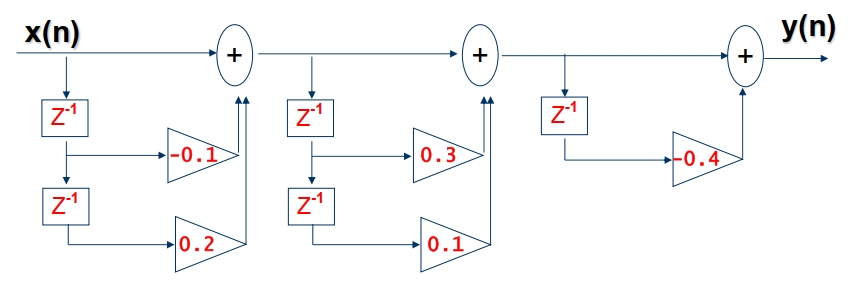
\includegraphics[width=0.8\textwidth]{chap4/img/serial_flow_chart.png}
        \caption{例 \theexample~ 的级联流图}
        \label{fig:serial-flow-chart}
    \end{figure}
\end{example}

\begin{solution}
    不妨设 $x(n) = x_1(n), y(n) = y_3(n)$,
    以及 $y_1(n) = x_2(n), y_2(n) = x_3(n)$,则如图 \ref{fig:serial-flow-chart-annotated} 所示,
    \begin{align*}
        y_1(n) & = x_1(n) - 0.1x_1(n - 1) + 0.2x_1(n - 2), \\
        y_2(n) & = x_2(n) + 0.3x_2(n - 1) + 0.1x_2(n - 2), \\
        y_3(n) & = x_3(n) - 0.4x_3(n - 1).
    \end{align*}
    \begin{figure}[H]
        \centering
        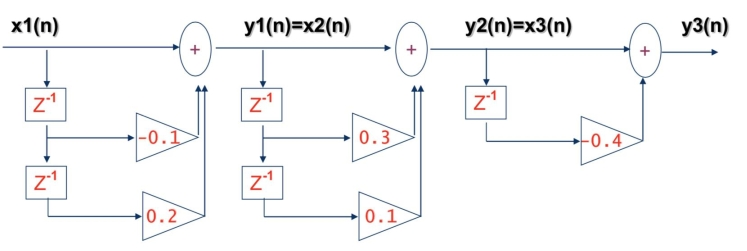
\includegraphics[width=0.8\textwidth]{chap4/img/serial_flow_chart_annotated.png}
        \caption{例 \theexample~ 的级联流图(带标注)}
        \label{fig:serial-flow-chart-annotated}
    \end{figure}
    将 $y_1(n)$ 代入 $y_2(n)$ 的表达式中,将 $y_2(n)$ 代入 $y_3(n)$ 的表达式中,
    可得级联流图的差分方程为
    \begin{align*}
        y_3(n) = x_1(n) - 0.2x_1(n - 1) + 0.19x_1(n - 2) - 0.058x_1(n - 3) - 0.008x_1(n - 5).
    \end{align*}
\end{solution}

\begin{exercise}
    \label{exercise:LTI-stable}
    证明:某 LTI 系统稳定的充要条件是
    \begin{align*}
        \sum_{n = -\infty}^{\infty} |h(n)| = P < \infty.
    \end{align*}
    其中 $h(n)$ 为系统的单位脉冲响应,$P$ 为一个常数。
\end{exercise}
